
\documentclass[12pt]{article}
%\documentclass{abnt}

\usepackage[brazil]{babel}
\usepackage[T1]{fontenc}
\usepackage[utf-8]{inputenc}
\usepackage{hyperref}
\usepackage{times}
\usepackage{listings}
\usepackage[dvips]{graphicx}

% \usepackage{abntex}

%\citeoption{abnt-full-initials=yes}
\lstset{language=ruby,caption=Código Ruby,label=Ruby, numbers=left} 

\title{Expressividade da linguagem enquanto programando}

\author{Jônatas Davi Paganini}

\date{novembro de 2009}

\begin{document}
\maketitle
\begin{abstract}
Este trabalho busca trazer ao leitor um ambiente de programação mais próximo de sua realidade. Através de exemplos de programas de computador, será mostrado como a linguagem de programação pode ser expressiva e de fácil compreensão.
\end{abstract}

\tableofcontents

\section{Teoria da linguagem}

Linguagem é qualquer e todo sistema de signos que serve de meio de comunicação de idéias ou sentimentos através de signos convencionais, sonoros, gráficos, gestuais etc., podendo ser percebida pelos diversos órgãos dos sentidos, o que leva a distinguirem-se várias espécies de linguagem: visual, auditiva, tátil, etc., ou, ainda, outras mais complexas, constituídas, ao mesmo tempo, de elementos diversos.12 Os elementos constitutivos da linguagem são, pois, gestos, sinais, sons, símbolos ou palavras, usados para representar conceitos de comunicação, idéias, significados e pensamentos. Embora os animais também se comuniquem, a linguagem propriamente dita pertence apenas ao Homem.

\cite{wikiLinguagem}

\section{Evolução da linguagem de programação}

A evolução dos computadores trouxe dispositivos menores e mais potentes. Na década de 80, usavam-se grandes computadores para realizar pequenos processos, 30 anos mais tarde estes dispositivos ganharam velocidade, design e consomem pouca energia. Dispositivos que cabem na palma da mão, com apenas alguns toques ou cliques tornam acessível a informação desejada. 

Da mesma forma,os computadores ganharam potência, as linguagens de programação se tornaram expressivas e humanas. Este dinâmismo não tem o objetivo de trazer conforto a máquina, mas sim ao seu manipulador - o homem. 

A linguagem de computador, inicialmente era grosseira e de difícil compreensão, com o passar do tempo, as técnicas foram evoluindo e a linguagem, mesmo de computador, foi ganhando forma e expressão. Houve uma percepção de mudança, que tornaria a linguagem de programação uma auxiliadora do programador e não uma interpretadora.

Uma linguagem tem os seus limites, na maioria dos casos é formal e burocrático. A linguagem Ruby quebra esta formalidade, torna o processo de codificação simples e livre. Em outras palavras, ela não bloqueia o trabalho do programador.

\subsection{Exemplo 'Hello world'}

   O programa Hello world é o programa mais conhecido no mundo inteiro e é o exemplo mais básico de uma linguagem de programação com o objetivo de imprimir a mensagem "Hello, world!" e guiar o iniciante em sua primeira compilação/execução de um programa de computador. Abaixo seguem dois exemplos "Hello, world" em duas linguagens de programação distintas: asssembly e ruby.


\subsubsection {Exemplo usando a linguagem de programação assembly}

\begin{lstlisting}[caption=Exemplo em assembly]

   variable:
      .message   db   "Hello world!\$"
   code:
      mov  ah,9
      mov  dx,offset .message
      int  0x21
      ret

\end{lstlisting}

Analisando a listagem 1.1 vemos que possuem muitas palavras (comandos, declarações) desconhecidas, e  com pouca aparência semântica. Isto acontece devido ao tipo de compilador (de linguagem compilada) e o nível de acesso as complexidades do hardware do computador. 

\subsubsection {Exemplo usando a linguagem de programação ruby}

\begin{lstlisting}[caption=Exemplo em ruby]
   print "Hello, world!"
\end{lstlisting}

\subsection { A simplicidade da linguagem }

Foi necessário apenas uma linha de código para representar o mesmo exemplo na linguagem ruby. No exemplo mais simples o objetivo é apenas imprimir "Hello, world!" e é exatamente isso que está escrito. Diferente de assembly, ruby não é uma linguagem compilada e sim dinâmica. Assim, tudo acontece em tempo real, enquanto está sendo executado.
   
\begin{lstlisting}[caption=Tradução do programa ruby]
   imprima "Ola mundo!"
\end{lstlisting}

Apenas com uma linha de código é possível fazer exatamente o que está sendo proposto. Este programa de computador foi escrito de forma simples e humanamente legível, diferente da primeira instrução de máquina escrita em assembly. No decorrer deste artigo serão abordados outros exemplos de programação como este, que, com poucas palavras expressa exatamente o objetivo do software no domínio em questão.
Exemplos como este, mostram o poder do homem de categorizar e generalizar as informações. Desta forma a percepção mudou de, programar para o computador para programar para as outras pessoas. Anteriormente, com uma programação rígida e a escassez de processamento, a codificação de um software realmente fazia parte de um processo árduo e lento, aonde não era possível tornar agradável a leitura de uma instrução de computador.



\section { A linguagem ruby }

Ruby é uma linguagem dinâmica, open source com foco na simplicidade e produtividade. Tem uma sintaxe elegante de leitura natural e fácil escrita. Com um grande número de bibliotecas disponíveis gratuitamente (gems), tem atraído muita gente para desenvolver nesta linguagem.

Para usar no Mac OS X ou Linux, é necessário abrir o {terminal} e  no Windows pode-se usar o Command-DOS e após isso digitar ruby para invocar o compilador, irb para iniciar uma interação.

\subsection { O compilador ruby }

O compilado pode ser invocado usando a linha de comando e receber uma código para compilar"

\begin{lstlisting}[caption=Usando o compilador na linha de comando]
jonatas@xonatax-mac:~$ ruby -e "puts 1+2"
3
\end{lstlisting}

\subsection { Ruby Interativo - IRB }

Existe um programa chamado IRB, que vem instalado com compilador de ruby, que serve para interagir com a linguagem na forma de console. As linhas do console ruby digitadas são iniciadas por >> e as linhas que trazem o resultado da expressão são iniciadas por =>. Estes símbolos não fazem parte do código de programação, apenas identificam a situação do terminal interativo.

\begin{lstlisting}[caption=Usando o compilador na linha de comando]
jonatas@xonatax-mac:~$ irb
>> 1.class
=> Fixnum
>> 1 + 2
=> 3
\end{lstlisting}

\subsection { Tipos de dados }

\subsubsection { Strings }

As strings podem ser limitados por vários delimitadores, em geral são usadas aspas simples e duplas, mas existem outras formas.

\begin{lstlisting}[caption=Exemplos de uso de string]
>> " outra string" + ' mais uma' + %[ outra ]
=> " outra string mais uma outra "
\end{lstlisting}

\subsubsection { Números }

Os números são objetos como qualquer outro e os operadores são simples métodos.

\begin{lstlisting}[caption=Exemplos de uso de números ]
>> 1.class
=> Fixnum
>> 1.class.ancestors
=> [Fixnum, Integer, Precision, Numeric, Comparable, Object, Kernel]
>> 1.0.class
=> Float
\end{lstlisting}

\subsubsection { Hashes }

Este tipo de elemento que amarzena valores como uma matriz, mas é possível acessar os valores através de uma chave. O valor do elemento é indicado apartir da expressão:

\begin{lstlisting}[caption=Syntaxe do hash ]
{ :chave => valor }
\end

\begin{lstlisting}[caption=Exemplos de uso de hashes ]
sexo = { "M" => "Masculino", "F" => "Feminino"}
sexo["M"] # => "Masculino"
\end{lstlisting}

\subsubsection { Entrada de dados }

No exemplo abaixo será feito uma pergunta para o usuário e quando ele confirmar a resposta irá saudar o usuário.

\begin{lstlisting}[caption=Exemplo de entrada de dados ]
 print "qual seu nome?"
 nome = gets
 print "oi #{nome}"
\end{lstlisting}
 
Na primeira linha, é impressa a pergunta. Na próxima linha é atribuido a uma variável nome a entrada de dados dada pelo método gets.
Em seguinda é impressa a saudação oi juntamente com a variável nome. Notem que o uso de \#\{\} embutido na string já concatena a expressão interna a string.

\subsubsection { Métodos }

Os métodos podem ser usados apartir de uma classe, ou estarão definidos no módulo Kernel. Métodos são formas de interagir com o ambiente atual e encapsulam a função com parâmetros.

\begin{lstlisting}[caption=Exemplo de método ]
def ligar_para(telefone)
  puts "ligando para #{telefone}"
end
\end{lstlisting}

\subsection { Classes e Módulos }
 
Classe é a declaração que permite definir uma classe marcado pela palavra \textit{class} seguido do nome de elementos. Após isso, vem o corpo com as definições do corpo. O fim do corpo é marcado pela palavra end.

Módulos permitem dividir comportamentos de classe e de instância, permitindo assim a multipla extensão de classes. Ele pode ser usado em blocos e sub-blocos e todo o código gerado fica encapsulado na declaração. Esse recurso também pode ser usado para agrupar classes do mesmo gênero. 

\begin{lstlisting}[caption=Exemplo de módulo ]
  module Mamifero
    def mamar
      print "mamando..."
    end
  end
  class Gato
    include Mamifero
    def miar
       print "meauuuu"
    end
  end
\end{lstlisting}

Os módulos também são uma boa possibilidade para criar espaços de nomes. Com este recurso é possível trabalhar com nomes específicos e sem repetições de nomes.

No exemplo acima, é definido um módulo Mamifero está sendo declarado os seus recurso internos. Um módulo não pode ser instanciado, ele é apenas usado como um espaço de nomes. O objetivo dele é organizar pequenos comportamentos que podem ser utilizados em outros momentos.

\begin{lstlisting}[caption=Exemplo de módulo como espaço ]
module Condominio
  include PortaoEletronico
  class Apartamento
   # ... define o apartamento internamente
  end
end 
\end{lstlisting}

\subsection{ Variáveis } 

Quando iniciados com apenas um arroba (@), indicam ser uma variável de instância. Diferente de Java e muitas outras linguagens, não é necessário declarar a variável antes de usa-la. Elas simplesmente criam a referência logo na primeira vez que são usadas.
As variáveis locais são iniciadas por letras ou \textit{underscore}.
A atribuição de um valor a uma variável é feita através do sinal de igualdade (=).

\begin{lstlisting}[caption=Exemplo de variável local ]
meu_nome = "Jonatas"
\end{lstlisting}

A leitura da expressão acima seria: meu nome (a variável) é igual a Jonatas.
Em uma classe, as váriaveis são usadas como atributos internos.

\begin{lstlisting}[caption=Exemplo de variável de instância em uma classe ]
class Pessoa
  def initialize(nome)
    @nome = nome
  end
  def saudar
    puts "ola #{@nome}"
  end
end
\end{lstlisting}

O código acima pode ser usado da seguinte forma:

\begin{lstlisting}[caption=Exemplo de utilização da classe descrita acima ]
jonatas = Pessoa.new "Jonatas"
jonatas.saudar 
\end{lstlisting}

\subsubsection { Blocos de código }

\cite{programmingRuby}
Segundo Dave Thomas, todo mundo já quiz implementar o seu próprio recheio de método na sua própria estrutura. Um bloco pode ficar entre chaves ou entre as palavras \textit{ do } e \textit{ end }.

\begin{lstlisting}[caption=Exemplo de bloco de código ]
   5.times { print "hello word" }
\end{lstlisting}

Traduzindo: 
\begin{lstlisting}[caption=Exemplo de bloco de código ]
   5.vezes { imprima "ola mundo" }
\end{lstlisting}

O bloco de código é extensamente utilizado em \textit{frameworks} para apenas criar a estrutura e tornar óbvio o objetivo da linguagem.



\section{ Shoes }

\subsection{O que é Shoes?}

Shoes é um framework para a construção de interfaces rápidas. Shoes nasceu pra ser fácil. Realmente feito para iniciantes absolutos. Com esta ferramenta é realmente fácil de fazer interfaces e artes gráficas. 
Esta ferramenta permite criar interfaces desktop para todas as plataformas e muitos divertidas de aprender.

\subsection{ Exemplo de expressividade - janela com botão }

Este é um dos exemplos mais simples do shoes. 

\begin{lstlisting}[caption=Primeiro exemplo do framework Shoes  ]
Shoes.app { 
  button("Click me!") {
     alert("Good job.") 
  }
} 
\end{lstlisting}

Este programa foi escrito em uma linguagem chamada Ruby. Consiste em uma janela com um botão. Quando o botão for clicado ela deverá responder por: "Good job." ou seja "Bom trabalho."

Shoes roda na maioria das plataformas operacionais. Isto é ótimo pois é possível escrever apenas uma vez e usar no Linux, Mac OS X, Windows e muitos outros.

%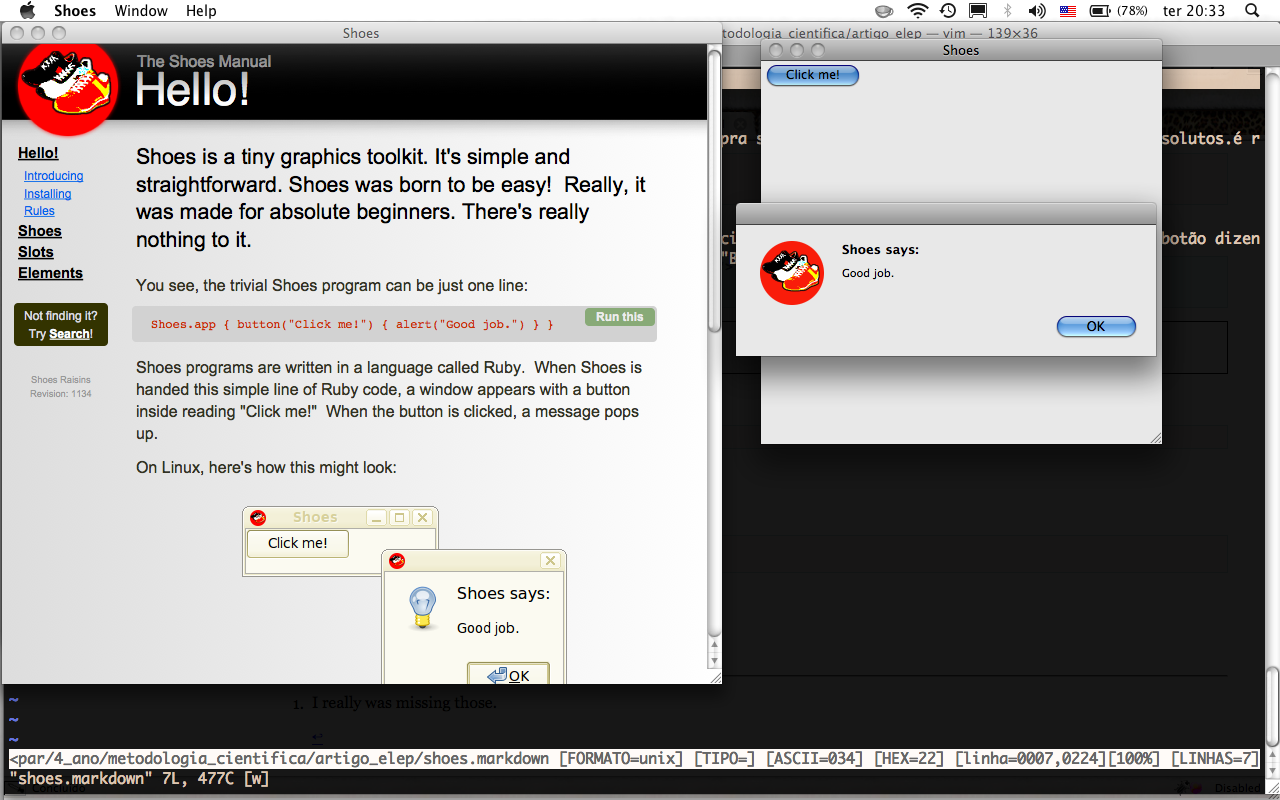
\includegraphics[scale=0.6]{shoes_hello_world.eps}
% (exemplo rodando no Mac OS X)!

\subsubsection{ Exemplo de expressividade - um bloco de notas com Shoes }

Como próximo exemplo, será progamado um bloco de notas que possa apagar e inserir novas notas em uma janela. O programa será composto por:
\begin{itemize} 
  \item uma janela com um título "Minhas Notas", tamanho 300 pixels. E dentro desta janela terá 
  \begin{itemize} 
    \item uma linha de edição para escrever a nota
    \item um botão para adicionar a anotação que quando for clicado deve 
    \begin{itemize} 
      \item adicionar o que foi escrito na linha de edição para as notas abaixo listadas
      \item limpar o texto da linha de edição da nota
    \end{itemize} 
  \end{itemize} 
  \item cada nota adicionada deve conter um link para remover a nota \ldots
\end{itemize} 


\subsection { Funcionamento do framework }

Como descrito na primeira linha de código do exemplo anterior, o framework é declarado, contendo uma janela principal. Esta janela, recebe um título e um tamanho inicial.
A declaração:

\lstinputlisting{shoes_tarefas.rb} 

Shoes.app inicia um aplicativo do framework, e dentro do corpo deste método é possível empilhar e enfileirar objetos. Com suas definições específicas de janela, também pode receber parâmetros. Este objeto pode encaixar muitos outros componentes internamente. Também é possível manipular elementos de fora para dentro, e de dentro para fora, fazendo com que um bloco interfira no outro sem dificuldades.

Como o exemplo acima mostra, o framework Shoes basicamente é uma pilha de componentes, podendo adicionar, empilhar e remover elementos com facilidade e clareza. Estes elementos quando empilhados, podem interagir apenas empilhados ou empilhados e aninhados a outras pilhas de elementos. 


\begin{lstlisting}[caption=Primeira explicação do framework Shoes  ]
Shoes.app :title => "Minhas Notas", :width => 480
\end{lstlisting}

Estes parâmetros como título(title) e tamanho(width) são pertencentes a janela principal do aplicativo, e podem ser acompanhados de outros como bloqueio de redimensionamento de janela.

Os parâmetros no formato chave e valor facilitam o uso e a extensão das possibilidades para cada elemento.

Na segunda linha do código existe a declaração do elemento da interface edit\_line que é responsável pela linha de edição que permite a entrada de dados. 

\begin{lstlisting}[caption=Entendendo a linha de edição]
@anotacao = edit_line
\end{lstlisting}

Este método edit\_line retorna um componente do Shoes do tipo caixa de entrada de texto, e é possível acessar o valor do texto digitado através do atributo text. 

Desta forma é possível testar o funcionamento do texto que está no input com um botão que quando pressionado exibe uma mensagem de alerta com a mensagem digitada:

\begin{lstlisting}[caption=Entendendo a linha de edição]
button("ver") { alert(@anotacao.text) } 
\end{lstlisting}


\bibliographystyle{amsalpha}
\begin{thebibliography}{9} 
\bibitem{wikiLinguagem} 
Wikipédia, 
Acesso em setembro de 2009.

\url{http://pt.wikipedia.org/wiki/Linguagem}

\bibitem{programmingRuby} 
Thomas, Dave. 
Programming Ruby: The Pragmatic programmers’ Guide. 
Segunda edição. Dallas, Texas: The Pragmatic Bookshelf, 2006.



\end{thebibliography} 

\end{document}


